\documentclass[12pt,twoside]{report}

%%%%%%%%%%%%%%%%%%%%%%%%%%%%%%%%%%%%%%%%%%%%%%%%%%%%%%%%%%%%%%%%%%%%%%%%%%%%%

% Definitions for the title page
% Edit these to provide the correct information
% e.g. \newcommand{\reportauthor}{Timothy Kimber}

\newcommand{\reporttitle}{Analysing property sales data using Data Science}
\newcommand{\reportauthor}{Wenxiang Luo}
\newcommand{\supervisor}{Chiraag Lala}
\newcommand{\degreetype}{MSc Computing}

%%%%%%%%%%%%%%%%%%%%%%%%%%%%%%%%%%%%%%%%%%%%%%%%%%%%%%%%%%%%%%%%%%%%%%%%%%%%%

% load some definitions and default packages
%%%%%%%%%%%%%%%%%%%%%%%%%%%%%%%%%%%%%%%%%
% University Assignment Title Page 
% LaTeX Template
% Version 1.0 (27/12/12)
%
% This template has been downloaded from:
% http://www.LaTeXTemplates.com
%
% Original author:
% WikiBooks (http://en.wikibooks.org/wiki/LaTeX/Title_Creation)
%
% License:
% CC BY-NC-SA 3.0 (http://creativecommons.org/licenses/by-nc-sa/3.0/)
% 
%
%%%%%%%%%%%%%%%%%%%%%%%%%%%%%%%%%%%%%%%%%
%----------------------------------------------------------------------------------------
%	PACKAGES AND OTHER DOCUMENT CONFIGURATIONS
%----------------------------------------------------------------------------------------
\usepackage[a4paper,hmargin=2.8cm,vmargin=2.0cm,includeheadfoot]{geometry}
\usepackage{textpos}
\usepackage[numbers]{natbib} % for bibliography
\usepackage{tabularx,longtable,multirow,subfigure,caption}%hangcaption
\usepackage{fncylab} %formatting of labels
\usepackage{fancyhdr} % page layout
\usepackage{url} % URLs
\usepackage[english]{babel}
\usepackage{amsmath}
\usepackage{graphicx}
\usepackage{dsfont}
\usepackage{epstopdf} % automatically replace .eps with .pdf in graphics
\usepackage{backref} % needed for citations
\usepackage{array}
\usepackage{latexsym}
\usepackage[pdftex,pagebackref,hypertexnames=false,colorlinks]{hyperref} % provide links in pdf

\hypersetup{pdftitle={},
  pdfsubject={}, 
  pdfauthor={},
  pdfkeywords={}, 
  pdfstartview=FitH,
  pdfpagemode={UseOutlines},% None, FullScreen, UseOutlines
  bookmarksnumbered=true, bookmarksopen=true, colorlinks,
    citecolor=black,%
    filecolor=black,%
    linkcolor=blue,%
    urlcolor=black}

\usepackage[all]{hypcap}


%\usepackage{color}
%\usepackage[tight,ugly]{units}
%\usepackage{float}
%\usepackage{tcolorbox}
%\usepackage[colorinlistoftodos]{todonotes}
% \usepackage{ntheorem}
% \theoremstyle{break}
% \newtheorem{lemma}{Lemma}
% \newtheorem{theorem}{Theorem}
% \newtheorem{remark}{Remark}
% \newtheorem{definition}{Definition}
% \newtheorem{proof}{Proof}


%%% Default fonts
\renewcommand*{\rmdefault}{bch}
\renewcommand*{\ttdefault}{cmtt}



%%% Default settings (page layout)
\setlength{\parindent}{0em}  % indentation of paragraph

\setlength{\headheight}{14.5pt}
\pagestyle{fancy}
\renewcommand{\chaptermark}[1]{\markboth{\chaptername\ \thechapter.\ #1}{}} 

\fancyfoot[ER,OL]{\sffamily\textbf{\thepage}}%Page no. in the left on odd pages and on right on even pages
\fancyfoot[OC,EC]{\sffamily }
\renewcommand{\headrulewidth}{0.1pt}
\renewcommand{\footrulewidth}{0.1pt}
\captionsetup{margin=10pt,font=small,labelfont=bf}


%--- chapter heading

\def\@makechapterhead#1{%
  \vspace*{10\p@}%
  {\parindent \z@ \raggedright \sffamily
    \interlinepenalty\@M
    \Huge\bfseries \thechapter \space\space #1\par\nobreak
    \vskip 30\p@
  }}

%---chapter heading for \chapter*  
\def\@makeschapterhead#1{%
  \vspace*{10\p@}%
  {\parindent \z@ \raggedright
    \sffamily
    \interlinepenalty\@M
    \Huge \bfseries  #1\par\nobreak
    \vskip 30\p@
  }}

\allowdisplaybreaks

% load some macros
% Here, you can define your own macros. Some examples are given below.

\newcommand{\R}[0]{\mathds{R}} % real numbers
\newcommand{\Z}[0]{\mathds{Z}} % integers
\newcommand{\N}[0]{\mathds{N}} % natural numbers
\newcommand{\C}[0]{\mathds{C}} % complex numbers
\renewcommand{\vec}[1]{{\boldsymbol{{#1}}}} % vector
\newcommand{\mat}[1]{{\boldsymbol{{#1}}}} % matrix


\date{June 2022}

\begin{document}

% load title page
% Last modification: 2015-08-17 (Marc Deisenroth)
\begin{titlepage}

\newcommand{\HRule}{\rule{\linewidth}{0.5mm}} % Defines a new command for the horizontal lines, change thickness here


%----------------------------------------------------------------------------------------
%	LOGO SECTION
%----------------------------------------------------------------------------------------


\includegraphics[width = 4cm]{./figures/imperial}\\[0.5cm] 

\center % Center remainder of the page

%----------------------------------------------------------------------------------------
%	HEADING SECTIONS
%----------------------------------------------------------------------------------------

\textsc{\Large Imperial College London}\\[0.5cm] 
\textsc{\large Department of Computing}\\[0.5cm] 

%----------------------------------------------------------------------------------------
%	TITLE SECTION
%----------------------------------------------------------------------------------------

\HRule \\[0.4cm]
{ \huge \bfseries \reporttitle}\\ % Title of your document
\HRule \\[1.5cm]
 
%----------------------------------------------------------------------------------------
%	AUTHOR SECTION
%----------------------------------------------------------------------------------------

\begin{minipage}{0.4\textwidth}
\begin{flushleft} \large
\emph{Author:}\\
\reportauthor % Your name
\end{flushleft}
\end{minipage}
~
\begin{minipage}{0.4\textwidth}
\begin{flushright} \large
\emph{Supervisor:} \\
\supervisor % Supervisor's Name
\end{flushright}
\end{minipage}\\[4cm]


%----------------------------------------------------------------------------------------
%	FOOTER & DATE SECTION
%----------------------------------------------------------------------------------------
\vfill % Fill the rest of the page with whitespace
Submitted in partial fulfillment of the requirements for the MSc degree in
\degreetype~of Imperial College London\\[0.5cm]

\makeatletter
\@date 
\makeatother


\end{titlepage}



% page numbering etc.
\pagenumbering{roman}
\clearpage{\pagestyle{empty}\cleardoublepage}
\setcounter{page}{1}
\pagestyle{plain}
\graphicspath{ {./figures/} }

%%%%%%%%%%%%%%%%%%%%%%%%%%%%%%%%%%%%
\begin{abstract}
Your abstract.
\end{abstract}

\cleardoublepage
%%%%%%%%%%%%%%%%%%%%%%%%%%%%%%%%%%%%
\section*{Acknowledgments}
Comment this out if not needed.

\clearpage{\pagestyle{empty}\cleardoublepage}

%%%%%%%%%%%%%%%%%%%%%%%%%%%%%%%%%%%%
%--- table of contents
\fancyhead[RE,LO]{\sffamily {Table of Contents}}
\tableofcontents 


\clearpage{\pagestyle{empty}\cleardoublepage}
\pagenumbering{arabic}
\setcounter{page}{1}
\fancyhead[LE,RO]{\slshape \rightmark}
\fancyhead[LO,RE]{\slshape \leftmark}

%%%%%%%%%%%%%%%%%%%%%%%%%%%%%%%%%%%%
\chapter{Introduction}

Nowadays, there is a substantial amount of data generated every second. The daily lives of humans are producing it, and some other fields, such as research, health care, economic activities, and environmental information from various sensors, also generate a vast amount of data. Obtaining the relationship between some features or the patterns underlying these massive amounts of data might benefit the entire world. For instance, new causes of diseases might be identified, and technological advancement could be accelerated.
\\

However, this extensive data can be one of the main obstacles for analysis as it is approximately impossible for humans to obtain insights into the data manually. Under this circumstance, artificial intelligence (AI), a technique that empowers the computer to imitate human intelligence and manner,  could be one of the methods to mitigate this issue. It can extract patterns from large datasets and use them to make predictions based on future data and even identify which data components are responsible for the results.
\\

In this project, some AI techniques will be applied to property and demographic data to gain insights and understand the factors influencing a homeowner's likelihood to sell. The factors might include the proximity to schools, hospitals, or supermarkets, the accessibility to public transportation, and the property types (flats or houses). It could be highly advantageous to estate agents who would discover homeowners with more potential to become clients and provide them with business. 

\section{Aim \& Objective}
\section{Layout of the Report}

%%%%%%%%%%%%%%%%%%%%%%%%%%%%%%%%%%%%
\chapter{Literal Review}
Python is one of the most popular programming languages in the world since it is simple to develop, and there are extensive packages for various functionalities. In this project, Python and its packages would be used for loading data, preprocessing data, and constructing and evaluating machine learning models. 

\section{Machine Learning}
Machine Learning (ML), a subset of AI, is a technique that the computer can learn and improve from data without explicit programming. The reason for utilizing ML is that its performance is sometimes better than the conventional approach. For example, ML techniques would simplify the solution to a problem that comprises a long list of rules (spam mail detection). 
\\

ML can be divided into three categories, one of which is supervised learning. In supervised learning, the dataset contains features (input to the model) and targets (ground truth of the output), and the model's parameters are randomly initialized. Then the features are passed to the model, and the differences between the current output and the ground truth are used to update the parameters until the differences are acceptable. 
\\

In this project, a supervised learning model will be implemented for data analysis, and the steps are listed below.
\begin{enumerate}
	\item Data Preprocessing: Some data from the dataset may be missing, and these values must be handled appropriately before being passed to the model. 
	\item Standardization: In real life, different features usually have different ranges, and this will cause a problem in ML, which is that high magnitude features would have more weight than low magnitude features \citep{RN4}. One of the solutions is standardization, which could scale all the features to the same magnitude.
	\item Feature encoding: ML models require numerical values, whereas the categorical features in the dataset do not satisfy this requirement. Therefore, these features should be converted into numerical values. 
	\item Training \& Testing: The parameters of the model are updated, and it is expected that the loss will converge during training. The performance of the model is validated when testing.
\end{enumerate}

\section{Handle Text Information}
The format of texts in this project could be classified as HTML and plaintext. Although Python standard libraries provide some string processing capabilities, they are insufficient for this situation. 

\subsection{Beautiful Soup}
\textit{\textbf{Beautiful Soup}} is a Python library for extracting data from markup languages, such as HTML and XML. It can accomplish this with a user-specified parser, for example, \textbf{\textit{html.parser}}, to navigate, search and modify the parse tree, which would save considerable time \citep{RN10}. 

\subsection{parse}
The \textit{\textbf{format}} function in the Python standard library formats a string, whereas the \textit{\textbf{parse}} module provides functions with an oppositse effect, i.e., extract information from formatted strings.

\subsection{Regular Expression}
A regular expression is a sequence of ordinary and special characters representing textual patterns. The ordinary characters are identical throughout the expressions and texts, while the special characters specify the pattern, including number, location, and type of characters  \citep{RN14}. One of the primary disadvantages of the regular expression is its obscure syntax, which results in difficulty specifying a pattern. 

\subsection{Library Usage}
In this project, HTML texts are used extensively in the raw dataset to describe property summaries, property layouts, and council tax. This is the optimal scenario for \textit{Beautiful Soup} which is employed to extract plaintext by specifying tags. Then, \textit{parse} is applied to obtain the information, such as room names, from the plaintexts since they are in the same format. In addition, due to its limitations, the regular expression is only used to acquire numerical values in this project. 


\section{Data Manipulation}
\subsection{NumPy}
Numerical Python (\textit{\textbf{NumPy}}) is a scientific computing package designed to support large multidimensional matrices. It uses an optimized \textit{C/C++} API to reduce computation time compared to pure Python computations \citep{RN6}. A substantial number of complex tasks of data analytics can be simplified by numerous \textit{numpy} features. For example, it provides robust matrix operations, facilitates the construction of multidimensional objects, and serves as the foundation of other packages, including \textit{matplotlib} and \textit{seaborn}.

\subsection{Pandas}
The \textbf{\textit{pandas}} is an open-source and compelling package that was developed primarily for data analysis and data manipulation and is built on \textit{numpy}. It is capable of handling data of various types (numerical values, strings, and time) and from a variety of sources (CSV, Excel, and MqSQL database). \textbf{\textit{DataFrame}} is one of the \textit{pandas} data structures that is appropriate for handling tabular data with columns of different types. Additionally, it could manage various operations, such as manipulating missing values, creating pivot tables, and grouping data from different columns \citep{RN4}. 

\subsection{Library Usage}
In this project, the dataset provided is in CSV format hence it could be loaded by \textbf{\textit{Pandas}} since it is suitable for tabular data. Then the package is utilized for preprocessing, such as handling missing values and grouping columns of data. 
\\

\textit{\textbf{Numpy}} is appropriate for manipulating numerical data and acts as an intermediary between various packages. Therefore, it could be employed to evaluate the performance of ML models and transmit data to plotting packages. 


\section{ML Frameworks}
\subsection{Scikit-learn}
\textit{\textbf{Scikit-learn}} is a popular open-source ML framework that employs \textit{Numpy}. It contains traditional ML algorithms, including clustering, classification, and regression, as well as a variety of utilities that can be applied to preprocess data and evaluate the performance \citep{RN7}. The drawback of this library is that it does not natively support GPU acceleration and is not a neural network framework. 

\subsection{PyTorch}
\textbf{\textit{PyTorch}} is one of the popular ML frameworks developed by Facebook, which is designed to implement neural networks with flexibility and speed \citep{RN5}. It provides various components for model construction and training. For instance, there are numerous types of modules that comprise a model, such as linear layers, dropout, and activation functions, as well as a variety of loss functions and optimizers that can be employed in model training. 
\\

Furthermore, it can be beneficial to construct and train a model with \textit{Pytorch}. It has a Pythonic nature which means that its syntax is similar to Python, making it more straightforward for Python programmers to develop neural networks than other ML frameworks. Moreover, it is a rapidly expanding framework for developing neural networks with a vast ecosystem, meaning that a substantial number of utilities have been developed on top of it \citep{RN5}. Additionally, \textit{PyTorch} supports automatic differentiation and GPU acceleration which can be advantageous for model training.

\subsection{TensorFlow}
\textit{\textbf{TensorFlow}} is another ML framework produced by Google that specializes in deep learning and neural networks. It provides approximately the same components as \textit{PyTorch} and also supports automatic differentiation and GPU acceleration. One of the appealing characteristics of \textit{TensorFlow} is called \textit{\textbf{TensorBoard}}, which is an interactive visualization system that can display the flowchart of the data manipulation and plot the tendency of the performance \citep{RN15}. 

\subsection{Library Usage}
This project aims to construct a neural network which means \textit{scikit-learn} is not applicable at this stage. Although \textit{TensorFlow} provides the same capabilities as \textit{PyTorch} and is superior in visualization, the model construction and training will use \textit{PyTorch} due to its Pythonic syntax and compatibility with \textit{TensorBoard}. 
\\

However, \textit{scikit-learn} can be used to preprocess datasets and evaluate performance. It provides various utilities that can be helpful before training, for example, encoding categorical features and splitting the dataset into training and validation. In addition, it offers features for model evaluation, such as confusion matrix, accuracy, and recall. 

\section{Data Visualization}
\subsection{Matplotlib}
\textbf{\textit{Matplotlib}} is a Python package for 2D plotting that produces high-quality figures. It supports interactive and non-interactive plotting and can save images in multiple formats, including PNG and JPEG. It can also generate numerous types of graphs, such as line plots, scatter plots, and pie plots.

\subsection{Seaborn}
\textbf{\textit{Seaborn}} is a Python library for creating statistical graphs that integrates with \textit{pandas} to offer a high-level interface to \textit{matploblib}. If a dataset is provided, \textit{seaborn} can automatically generate the figure with appropriate plotting attributes, such as color and legend. Additionally, it is capable of generating comprehensive graphics with a single function call and a minimum number of arguments \citep{RN16}.

\subsection{Library Usage}
In this project, data visualization would be beneficial during preprocessing data and performance evaluation. For preprocessing, the distribution of the raw data should be inspected, hence \textit{seaborn} could be an optimal choice since the input is a \textit{DataFrame} and its syntax is concise. During evaluation, the model output will be converted to \textit{Numpy} arrays. Therefore, \textit{matplotlib} can be used in this case, as it is interactive and the figure can be further adjusted to illustrate the performance. 

\section{Methodology}

%%%%%%%%%%%%%%%%%%%%%%%%%%%%%%%%%%%%%%%%%%%%%%%%%%%%%%%%%%%%%%
\chapter{Implementation}
\section{Data Source and Collection}
The datasets used in this project are provided by EweMove, and transactions from 2018 to 2022 are included. There are 34591 records with 36 parameters describing each property after merging these datasets. Some parameters, such as postcodes, and room information, are independent variables that would be the model input. In contrast, the price and status of the transaction are dependent variables that serve as labels of supervised learning. The features that are used to train the model are listed in table \ref{model_input_features}. 

\begin{table}[h]
	\centering
	\caption{The features used to train the model}
	\label{model_input_features}
	\begin{tabular}{| l | l | l |}
		\hline
		\textbf{Feature} & \textbf{Description} & \textbf{Type} \\
		\hline
		Postcode & The location of the property & Categorical \\
		\hline
		Sale or Let & Whether the property is for sale or rent & Categorical \\
		\hline
		EweMove Description S3 Rooms & The room names and dimensions & HTML texts\\
		\hline
		RTD3308\_outside\_space & Keywords describing outside spaces & Categorical \\ 
		\hline
		RTD3307\_parking& Keywords describing parking & Categorical \\
		\hline
		RTD3316\_condition & The condition of the property & Categorical \\
		\hline
		RTD3318\_heating & Keywords describing heating & Categorical \\
		\hline
		RTD3317\_accessibility & Keywords describing accessibility & Categorical \\
		\hline
		Price / Rent & The price of the property & HTML texts \\
		\hline
		Price Qualifier & & Categorical \\
		\hline
		DESC Council Tax Band & Type of the council tax & Categorical \\
		\hline
		\# of Enquiry or viewings & Number of viewing inqueries & Numerical \\
		\hline
		\# of Apps/Offers & Number of offers & Numerical \\
		\hline
	\end{tabular}
\end{table}

\section{Data Preprocessing}

\subsection{Handle Room Descriptions (HTML)}
\subsubsection{Acquire room name and dimension}
The structure of the HTML texts containing the room information in a property is shown in figure \ref{html_structure}. The rooms are separated by tag \textit{$<$li$>$}, and the room name and its dimension is denoted by \textit{$<$strong$>$} and \textit{$<$i$>$} tags, respectively. Therefore, a function (\textit{\textbf{EweMove\_Description\_S3\_Rooms}}) was implemented to split the HTML texts by utilizing \textit{Beautiful soup}, and its flowchart is shown in figure \ref{html_room_info}.
\begin{figure}[h]
	\centering
	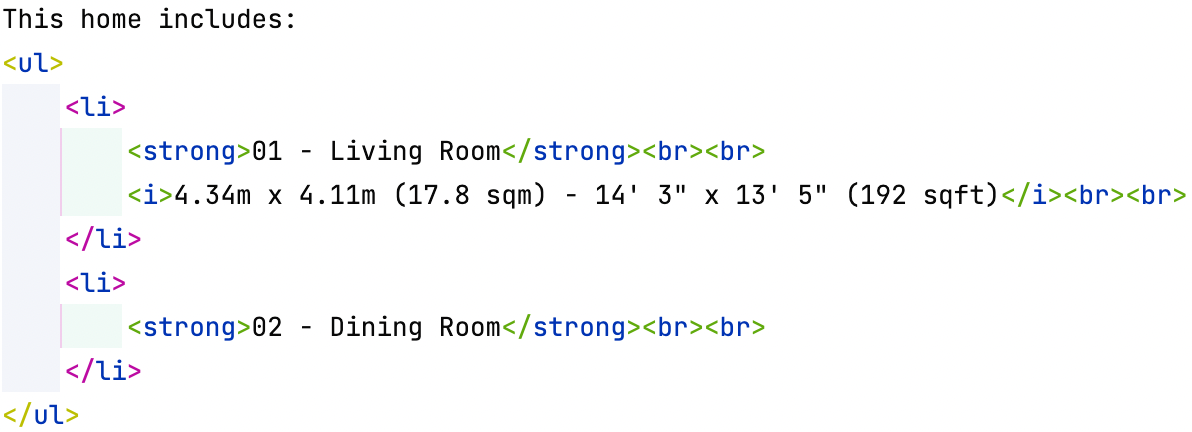
\includegraphics[width=15cm]{html_structure}
	\caption{The layout of HTML texts}
	\label{html_structure}
\end{figure}

\begin{figure}[h]
	\centering
	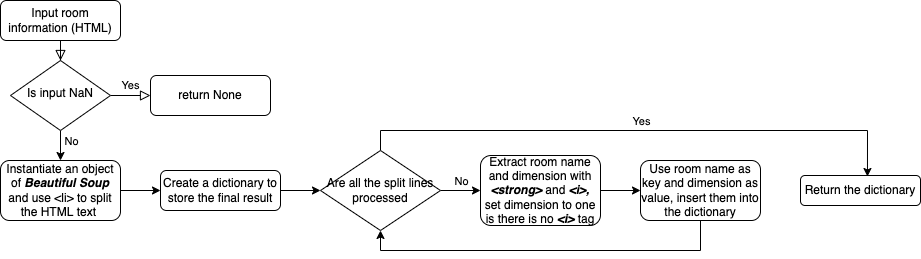
\includegraphics[width=1\linewidth]{html_room_info}
	\caption{Flowchart for extracting room information from HTML}
	\label{html_room_info}
\end{figure}

The names of rooms are analyzed after the room descriptions in the dataset have been processed. As a consequence, there are over 200 unique room names for approximately 36000 records, some of which are exceptionally uncommon across the entire dataset. For instance, only two properties have cinema rooms, and one has a lift, which is less than 0.1\% of all entries.  
\\

Due to the large number of room names, it is impossible to use it as the input of the model. Therefore, the rooms are divided into six categories: bedrooms, bathrooms, kitchens, living/reception rooms, dining rooms, and other rooms so that the data can be generalized. 
\\

\subsubsection{Generalize room information}
A class, \textit{\textbf{ExtractRooms}}, was developed to acquire and integrate the room information, especially the area in square meters, and its UML diagram is shown in figure \ref{uml_extract_rooms}. The member variable \textit{rooms} is a list containing the result of invoking \textit{EweMove\_Description\_S3\_Rooms}, \textit{room\_set} comprises all the room names, \textit{current\_rooms} consists of the room names that have been processed, and \textit{extract\_area} is a formatted string for acquiring room area. 
\\

\begin{figure}[h]
	\centering
	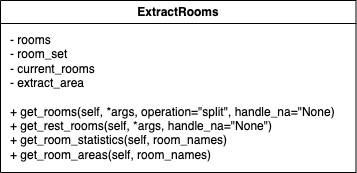
\includegraphics[width=10cm]{uml_extract_rooms}
	\caption{The UML diagram of the class (\textit{ExtractRooms})}
	\label{uml_extract_rooms}
\end{figure}

Key member functions
\begin{itemize}
	\item get\_rooms \\
	The flow diagram of this method is shown in figure \ref{extract_room_get_rooms} and the arguments are listed below.
	\begin{enumerate}
		\item args: It should be noted that this is a variable-length argument, which means that it can accept as many arguments as possible, and it is used to select room names from \textit{room\_set}. For instance, \textit{*args = [living, reception]} will select all names containing \textit{living} or \textit{reception}. 
		\item operation: The argumen determines the types of the final result and the valid inputs include \textit{sum}, \textit{mean}, \textit{split}, and \textit{number}. For example, if args is \textit{bedroom}, then the function can return the sum of bedroom areas, the average bedroom area, the area of each bedroom and the number of bedrooms. 
		\item handle\_na: This parameter specifies how to manage missing values, either by ignoring them or by filling the mean value if the input is \textit{None} or \textit{mean}, respectively. 
	\end{enumerate} 
	\begin{figure}[h]
		\centering
		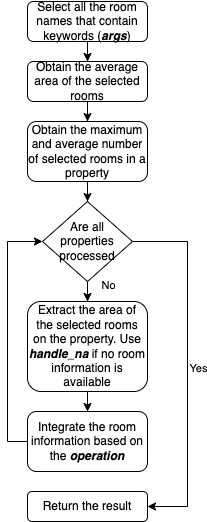
\includegraphics[height=11cm]{extract_room_get_rooms}
		\caption{Flowchart of \textit{get\_rooms}}
		\label{extract_room_get_rooms}
	\end{figure}
	\item get\_rest\_room: \\
	This method is identical to \textit{\textbf{get\_room}} with two exceptions. The parameter \textit{\textbf{*args}} is used to disgard the room names containing the keywords, and only the number and the total areas of other rooms are returned. 
\end{itemize}

\subsection{Manipulate Categorical Keywords}
In the dataset, four features are characterized by categorical keywords, including parking, heating, accessibility, and outdoor spaces. Figure \ref{parking_dataset} is a snippet of the parking dataset that is used as an example to illustrate the manipulation of the keywords. The first three rows indicate that there is a parking space for the first property, which is \textbf{allocated} \textbf{off-street} parking for \textbf{residents}, the second has none, and the third property has one \textbf{on-street} parking space. In this situation, feature encoding cannot be applied since there are multiple columns of keywords describing a feature, and the order and quantity of the keywords have no effect.

\begin{figure}[h]
	\centering
	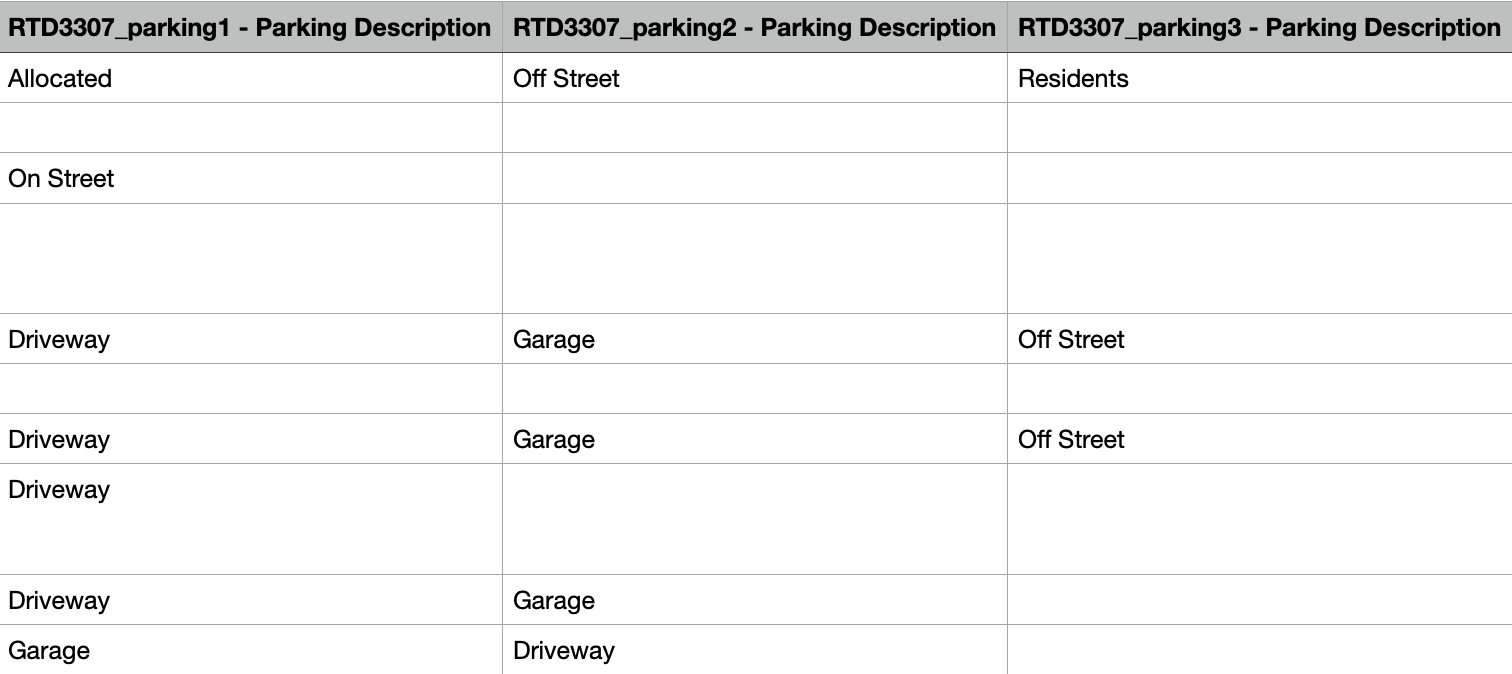
\includegraphics[width=12cm]{parking_dataset}
	\caption{The parking spaces in the first five properties}
	\label{parking_dataset}
\end{figure}

Figure \ref{uml_generalize_dataset} illustrates the UML diagram of the class \textit{\textbf{GeneralizeDataset}}, which was developed to determine how these features of each property are described and the number of keywords within the description. The core of this class is member function \textit{\textbf{get\_feature\_types}}, and its flowchart is displayed in figure \ref{generalize_dataset_get_feature_types}. In addition, function \textbf{\textit{get\_feature\_num}} can be used to determine the number of keywords for each property. 
\begin{figure}[h]
	\centering
	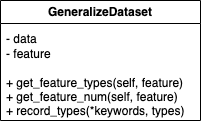
\includegraphics[width=5cm]{uml_generalize_dataset}
	\caption{The UML diagram of \textit{GeneralizeDataset}}
	\label{uml_generalize_dataset}
\end{figure}

\begin{figure}[h]
	\centering
	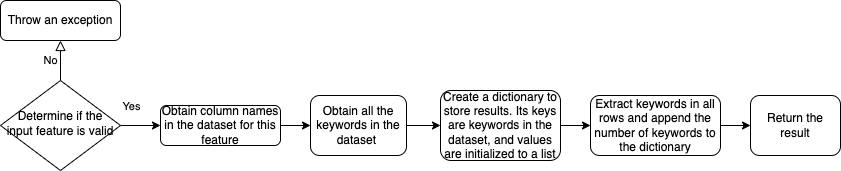
\includegraphics[width=1\linewidth]{generalize_dataset_get_feature_types}
	\caption{Flowchart of \textit{get\_feature\_types}}
	\label{generalize_dataset_get_feature_types}
\end{figure}

\subsection{Manage Outliers}
The price is crucial to the project, and the distribution of the raw data was inspected, as shown in figure \ref{price_raw}. The spike on the left side of the figure indicates that numerous properties have zero prices, which is illogical. Therefore, these abnormal values should be addressed as they could significantly impact the performance of the model.

\begin{figure*}[h]
	\centering
	\subfigure[All Prices]{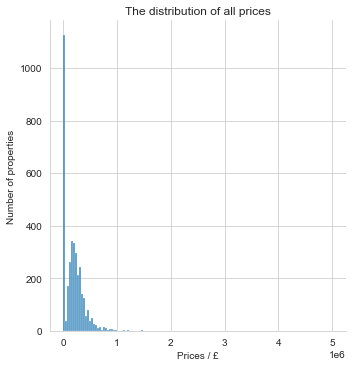
\includegraphics[width=5cm]{price_all_raw}\label{price_all_raw}}
	\hfill
	\subfigure[Sale Prices]{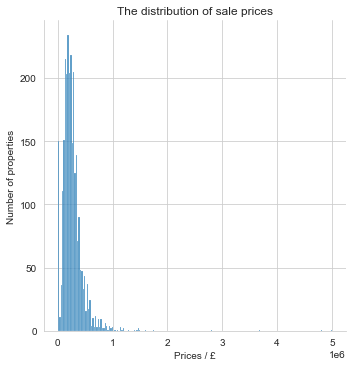
\includegraphics[width=5cm]{price_sale_raw}\label{price_sale_raw}}
	\hfill
	\subfigure[Rental Prices]{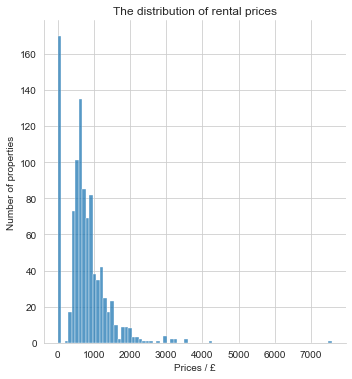
\includegraphics[width=5cm]{price_rental_raw}\label{price_rental_raw}}
	\caption{The distribution of prices from raw data}
	\label{price_raw}
\end{figure*}

\subsection{Create Input Dataset}

\subsubsection{Feature Encoding}
This technique is applicable to categorical features in the dataset, including price qualifier, council tax band, and property condition. The label encoding was employed, which is capable of converting the feature into numeric values between 0 and N - 1, where N is the number of distinct classes in a column.

\subsubsection{Manage Missing Values}
The datasets used in this project contain a significant number of missing values. For example, approximately 30\% of the room layout and more than 40\% of the council tax band are missing. Under this situation, it is impossible to replace them with the mean value  since it causes the model to focus on the average and result in low performance. Therefore, another approach was applied, which was removing the missing values in the datasets. 

\begin{figure}[h]
	\centering
	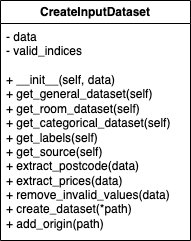
\includegraphics[height=6cm]{uml_create_input_dataset}
	\caption{The UML diagram of \textit{CreateInputDataset}}
	\label{uml_create_input_dataset}
\end{figure}

\subsubsection{Classy Approach}
After extracting the information from HTML texts and categorical keywords, it is combined with other columns in the dataset to produce a clean dataset for the model input.  Figure \ref{uml_create_input_dataset} is the UML diagram of \textit{\textbf{CreateInputDataset}}, which is a class developed for this objective, and the flow diagram of producing an input dataset is displayed in figure \ref{create_input_dataset}.

\begin{figure}[h]
	\centering
	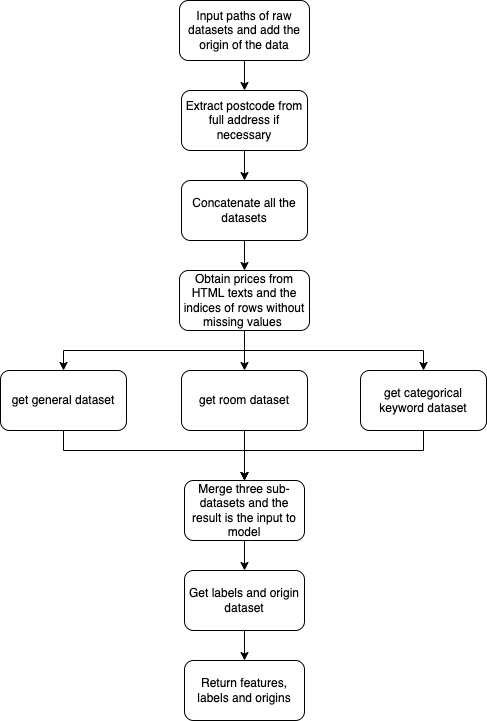
\includegraphics[height=7cm]{create_input_dataset}
	\caption{The flow diagram of producing  input dataset}
	\label{create_input_dataset}
\end{figure}

\section{Model Construction}

\subsection{Development Steps}
\subsubsection{Data Preparation}
The datasets created during preprocessing are initially loaded. Then they are split into training and testing sets, which represent 80\% and 20\% of the total dataset, respectively. In the meantime, the datasets are also shuffled as some datasets might contain intrinsic patterns.

\subsubsection{Training models}
Due to the limited training data for this project, cross validation was employed to train the model with different portions of training data. There are two model outputs, including prices and the status of transactions. The loss function for prices is mean squared error (MSE) as they are positive values. However, the status of transactions is either one or zero, hence its loss function is binary cross entropy (BCE). 
\\

The performance was illustrated after cross validation by plotting training and validation losses against epoch. Based on these graphs, the model with the best performance was selected for the evaluation phase. 

\subsubsection{Evaluation}
The model performance should be evaluated on unseen data. Otherwise, it would be useless. Various metrics are used to quantify the performance of the model in this project. 
\\

As the measurements for predicted prices, mean absolute error (MAE), mean squared error (MSE), and coefficient of determination ($R^2$) are applied.  The lower the MAE and MSE, the better the performance. $R^2$ values range from 0 to 1. A model with $R^2 = 0$ means the model cannot make accurate predictions, while $R^2 = 1$ indicates that the model can precisely predict the results. In rare instances, the $R^2$ can be negative, indicating that the model does not match the trend of the data, which is the worst performance. 
\\

The confusion matrix is initially obtained to access the predictions regarding the status of transactions. A confusion matrix summarizes the classification problems, indicating where the model outputs wrong predictions and the types of errors. Based on the confusion matrix, various metrics are calculated, and they are shown as follows, 
\begin{itemize}
	\item \textbf{Accuracy}: It is the number of correct predictions divided by the total number of predictions. The best accuracy is one and zero is the worst. 
	\item \textbf{Precision}: It is the number of correct positive predictions divided by the number of positive predictions. The best and worst precisions are one and zero, respectively. 
	\item \textbf{Recall}: the ratio of correct positive predictions to the total number of positive examples, and the high recall indicates that the class is correctly identified. 
	\item \textbf{F1 Score}: This is a harmonic mean of both recall and precision. Hence this value can be used to evaluate performance independently. 
\end{itemize}

\subsection{Linear Regression: Predict Price}
\label{linear_regression_model_construction}
Prior to the construction of any neural networks, a linear regression model with a single linear layer was developed. Its input size is the same as the number of features, and the output is the price. If this model can accurately predict the price, it eliminates the need to build more complex neural networks with multiple layers, which is the motivation for its creation. To train this model, Mean squared error (MSE) is applied as prices can be any positive values. The optimizer is Adam, and the learning rate is 0.001.  

\subsection{Basic Model: Output Sale Status and Price}
\label{basic_model_price_status_construction}
The architecture of this model only consists of linear layers and activation functions, as depicted in figure \ref{basic_model_layout}. There are two outputs of the model, which are prices and probabilities of selling. Therefore, the activation functions of the output layers are ReLU and sigmoid, respectively.
\\

The predicted probability should be converted into 0 or 1 to indicate the status of the transaction, given that it is either completed or not in the datasets. Therefore, a threshold of 0.5 is established. If the probability exceeds the threshold, then it is converted to 1. Otherwise, it is set to 0.
\\

The loss function for the status of the transaction is binary cross entropy (BCE), as it has only two possible outcomes. For the same reason as the linear regression model, MSE loss is applied to prices. Therefore, the total loss for this model is the sum of the BCE and MSE. In addition, the optimizer used for training is Adam, and the learning rate is 0.001. 
\\ 

\begin{figure}[h]
	\centering
	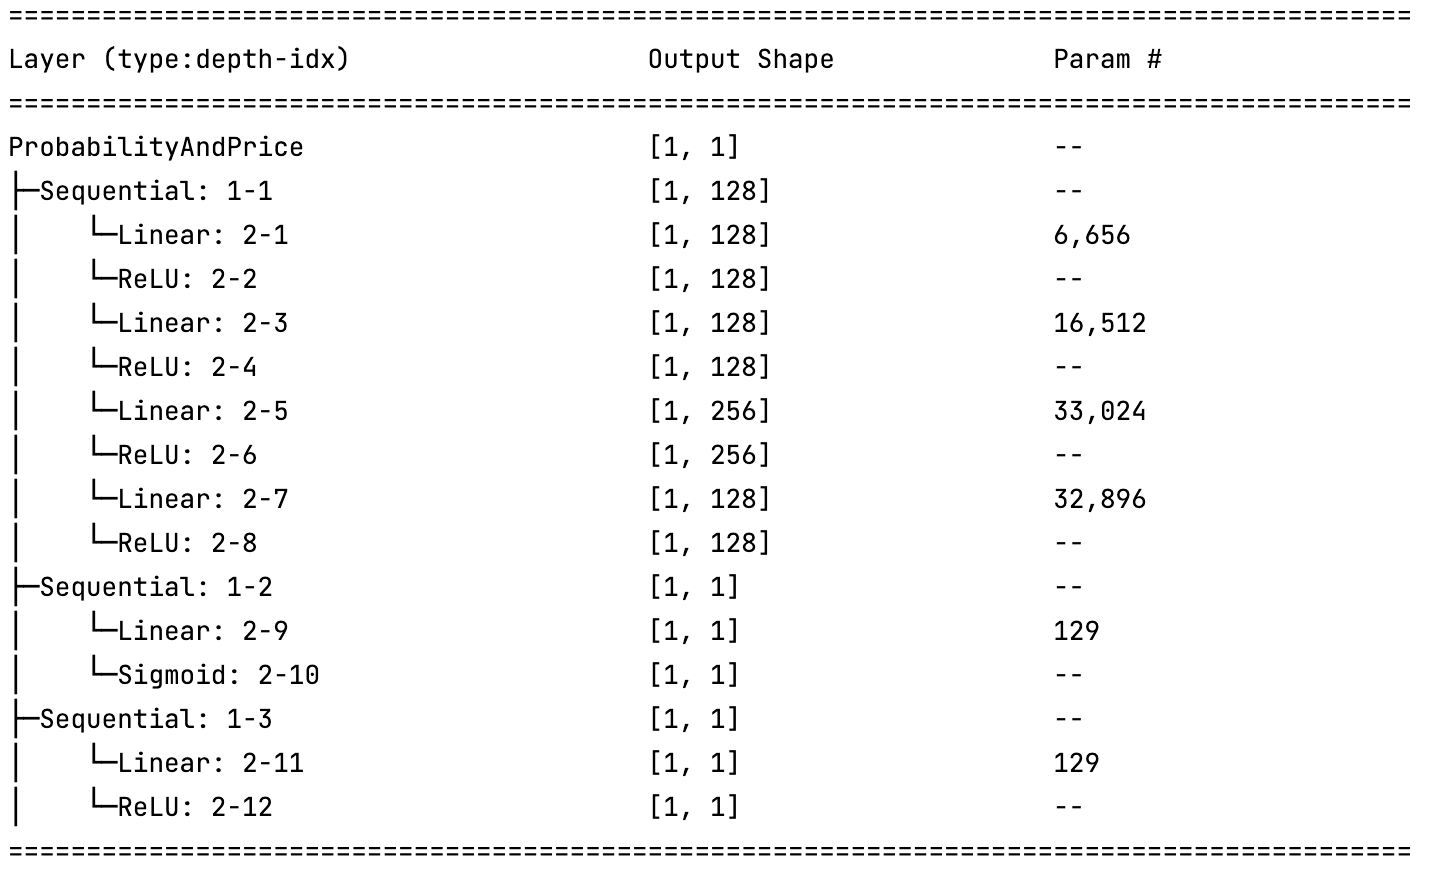
\includegraphics[width=1\linewidth]{basic_model_layout}
	\caption{The architecture of the basic model}
	\label{basic_model_layout}
\end{figure}

\subsection{Basic Model: Predicting Prices}
\label{basic_model_price_all}
The structure of this model is demonstrated in figure \ref{basic_model_price}. Its hidden layers are identical to the model for predicting completeness and prices, whereas the completeness output is removed. Due to this similarity, the optimizer and learning rate remain unchanged, and the loss function is MSE instead of the sum of BCE and MSE. 

\begin{figure}[h]
	\centering
	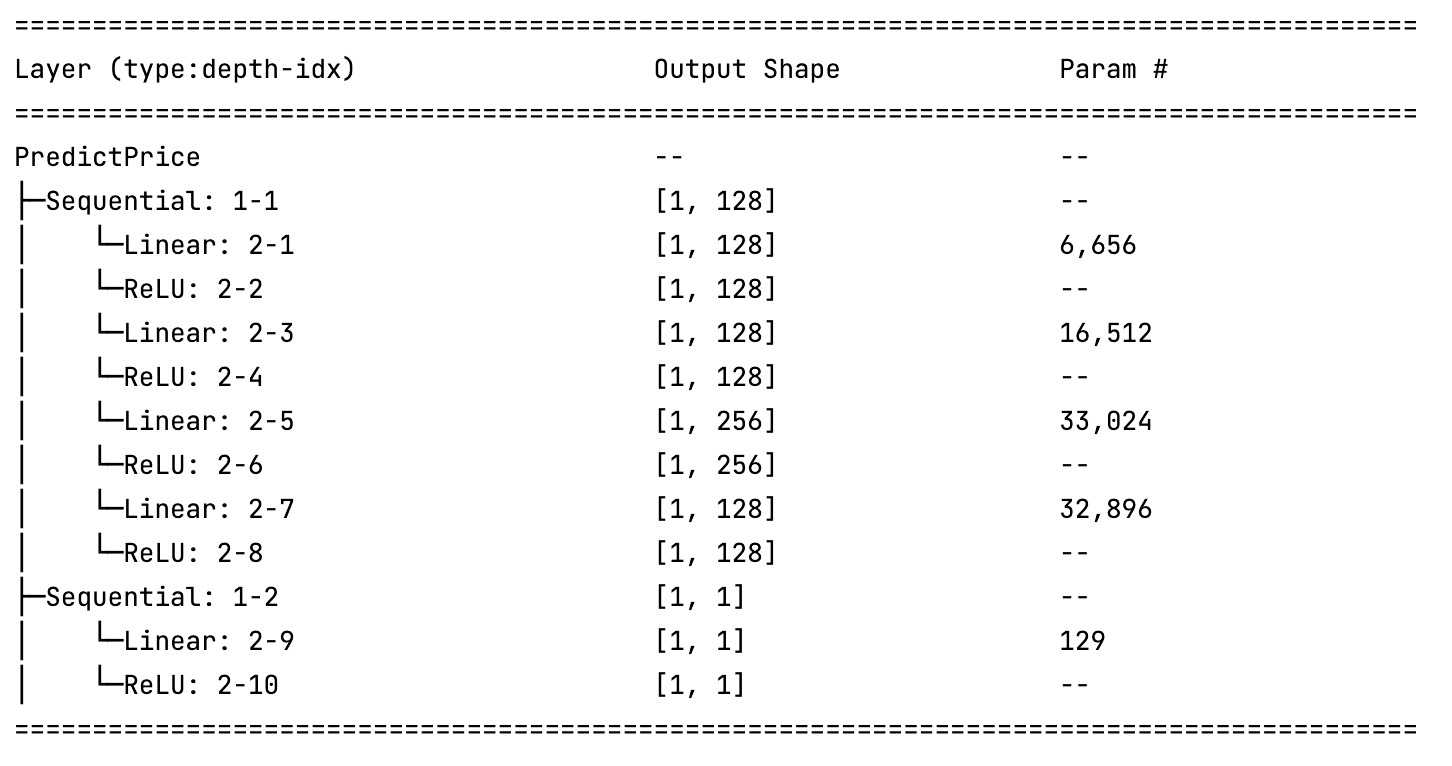
\includegraphics[width=1\linewidth]{basic_model_price}
	\caption{The structure of the basic model for predicting prices}
	\label{basic_model_price}
\end{figure}

%%%%%%%%%%%%%%%%%%%%%%%%%%%%%%%%%%%%%%%%%%%%%%%%%%%%%%%%%%%%%%%%%%%
\chapter{Testing \& Experimental Results}
Comprehensive testing and analyzing were conducted throughout the implementation but it is documented in this separate chapter for the sake of illuatration. 

\section{Data Preprocessing}

\subsection{Handle Room Descriptions (HTML)}
There were two tests for this objective, the first test examing if the room name and its dimension can be acquiare from HTML texts and the second test focuses on whether the room areas can be obtained and integrated correctly. 

\subsubsection{Acquire room name and dimension}
This test utilized two HTML texts, which are illustrated in figure \ref{html_room_info_test}. By invoking the function \textit{EweMove\_Description\_S3\_Rooms} with two snippets and retrieving the results (shown in tables \ref{html_room_info_expect_1} \& \ref{html_room_info_expect_2}), it is evident that the room names in two HTML snippets could be obtained, and the dimensions were acquired if available otherwise, the value was set to one. Therefore, this function can pass the test.

\begin{figure*}[h]
	\centering
	\subfigure[Snippte 1]{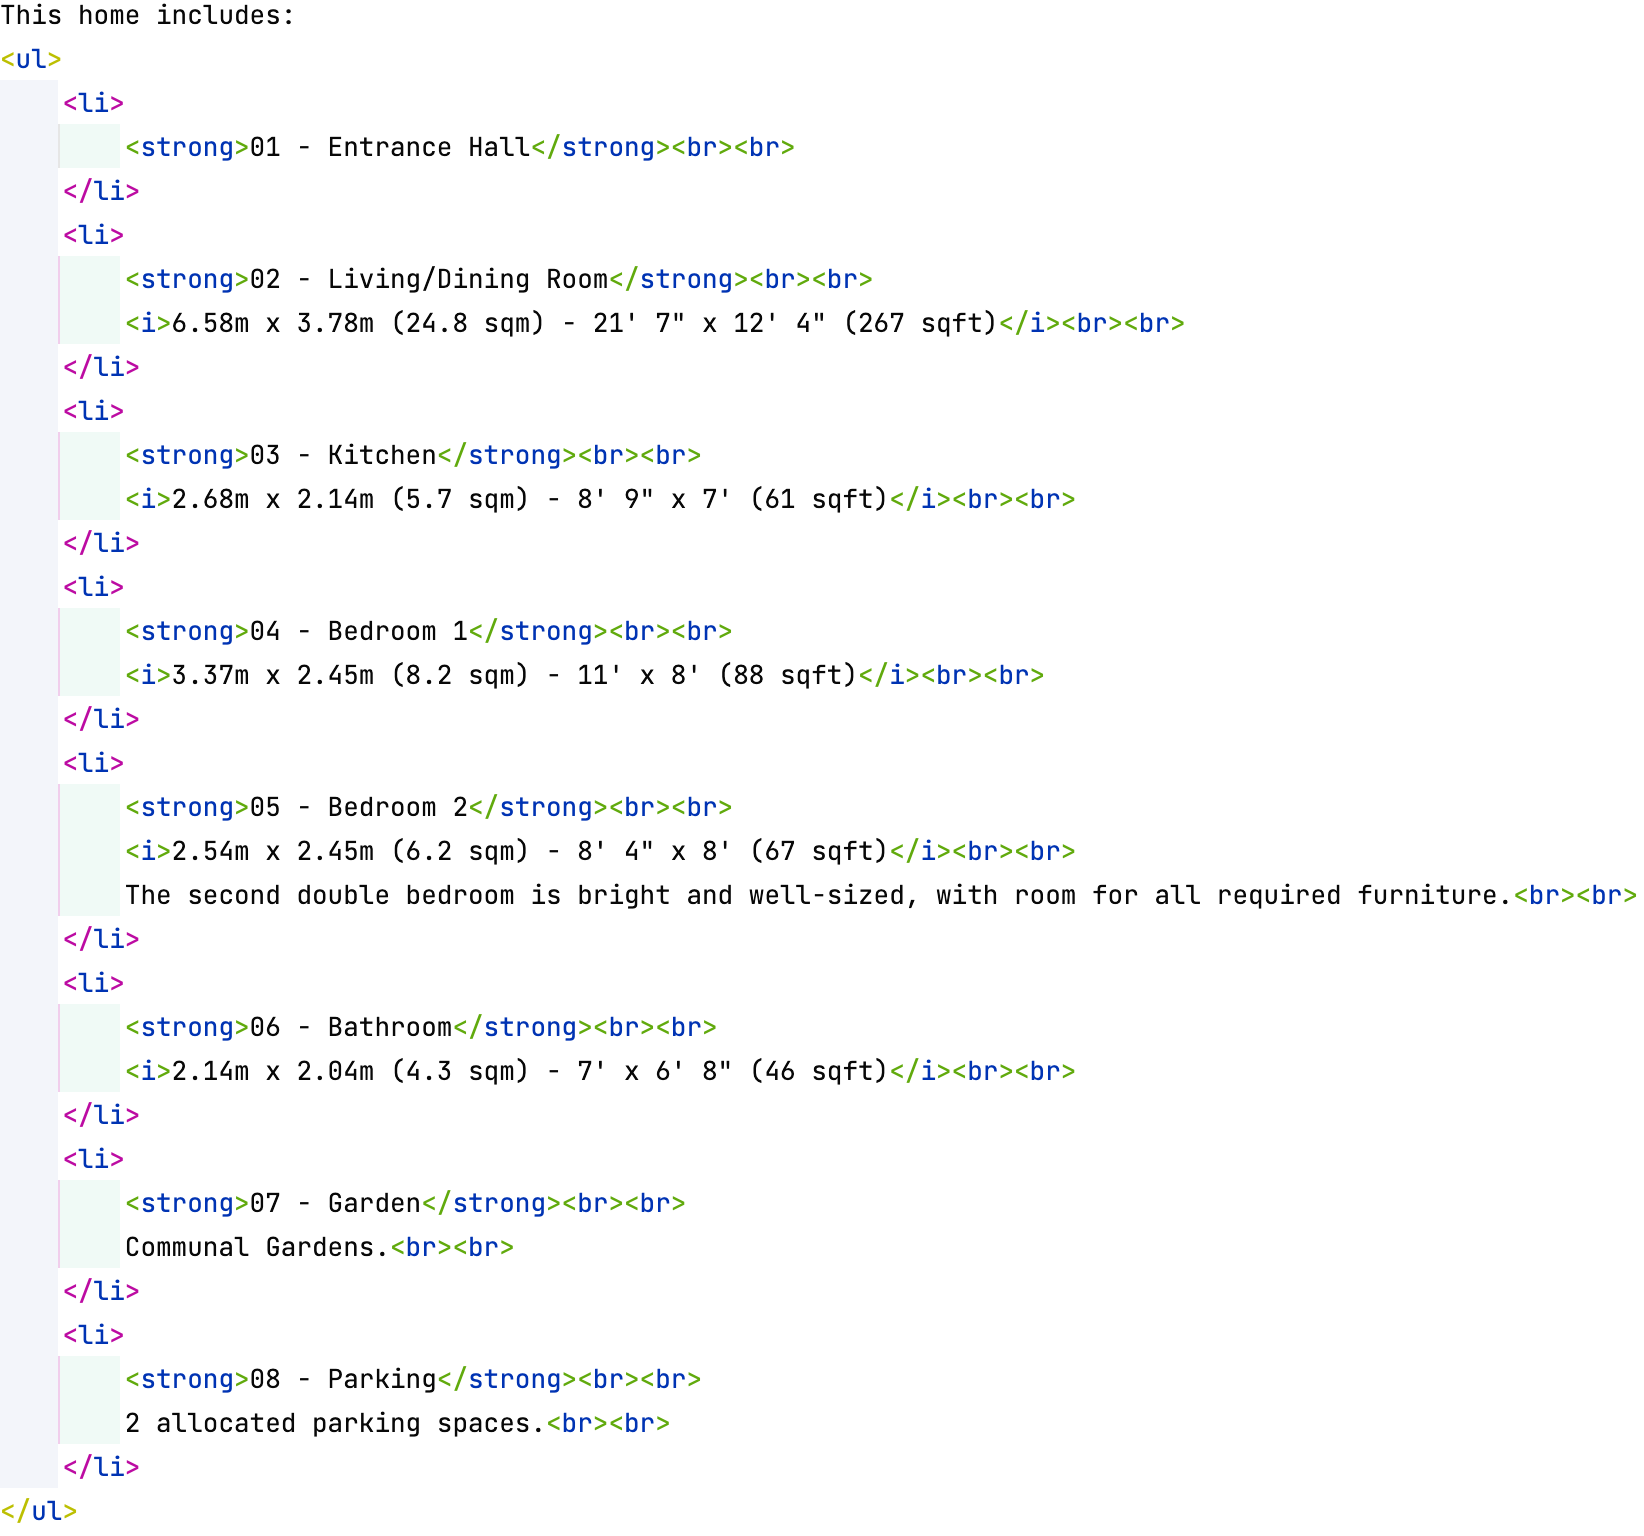
\includegraphics[width=7.5cm, height=8cm]{html_room_info_1}\label{html_room_info_test_1}}
	\hfill
	\subfigure[Snippet 2]{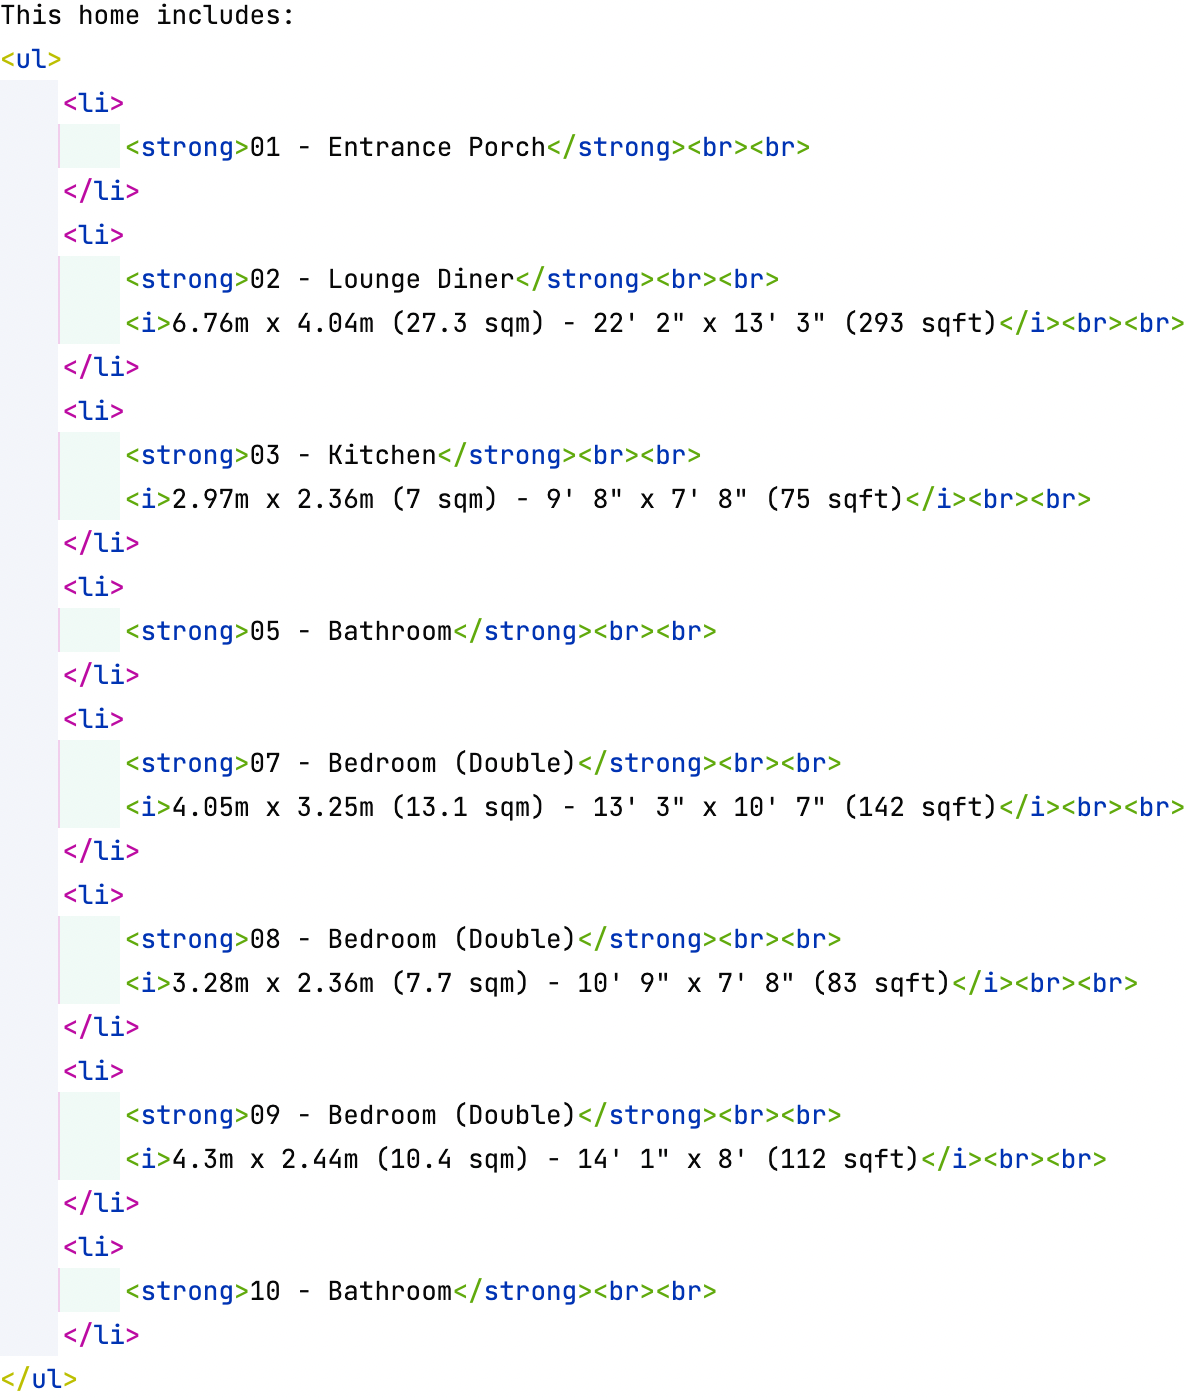
\includegraphics[width=7.5cm, height=8cm]{html_room_info_2}\label{html_room_info_test_2}}
	\caption{The HTML snippets for testing}
	\label{html_room_info_test}
\end{figure*}

\begin{table}[h]
	\centering
	\caption{Information from HTML snippet in figure \ref{html_room_info_test_1}}
	\begin{tabular} {| l | l |}
		\hline
		Entrance Hall & 1\\
		\hline
		Living/Dining Room & 6.58m x 3.78m (24.8 sqm) - 21' 7" x 12' 4" (267 sqft)\\
		\hline
		Kitchen & 2.68m x 2.14m (5.7 sqm) - 8' 9" x 7' (61 sqft)\\
		\hline
		Bedroom 1 & 3.37m x 2.45m (8.2 sqm) - 11' x 8' (88 sqft)\\
		\hline
		Bedroom 2 & 2.54m x 2.45m (6.2 sqm) - 8' 4" x 8' (67 sqft)\\
		\hline 
		Bathroom & 2.14m x 2.04m (4.3 sqm) - 7' x 6' 8" (46 sqft)\\
		\hline
		Garden & 1\\
		\hline
		Parking & 1\\
		\hline
	\end{tabular}
	\label{html_room_info_expect_1}
\end{table}

\begin{table}[h]
	\centering
	\caption{Information from HTML snippet in figure \ref*{html_room_info_test_2}}
	\begin{tabular} {| l | l |}
		\hline
		Entrance Porch & 1\\
		\hline
		Lounge Diner & 6.76m x 4.04m (27.3 sqm) - 22' 2" x 13' 3" (293 sqft)\\
		\hline
		Kitchen & 2.97m x 2.36m (7 sqm) - 9' 8" x 7' 8" (75 sqft)\\
		\hline
		Bathroom & 1\\
		\hline
		Bedroom (Double) & 4.05m x 3.25m (13.1 sqm) - 13' 3" x 10' 7" (142 sqft)\\
		\hline 
		Badroom (Double) & 3.28m x 2.36m (7.7 sqm) - 10' 9" x 7' 8" (83 sqft)\\
		\hline
		Bedroom (Double) & 4.3m x 2.44m (10.4 sqm) - 14' 1" x 8' (112 sqft)\\
		\hline
		Bathroom & 1\\
		\hline
	\end{tabular}
	\label{html_room_info_expect_2}
\end{table}

\subsubsection{Generalize room information}
The data obtained from HTML texts (figure \ref{html_room_info_test}) was used to access the behavior of \textit{ExtractRooms}, particularly its member function \textit{get\_rooms}. During testing, the selected type is the bedroom, and all the operations of \textit{get\_room} were inspected. Additionally, the other rooms were used to test function \textit{get\_rest\_rooms}. 
\\

The results of calling \textit{get\_rooms} are displayed in tables \ref{bedroom_info_split} and \ref{bedroom_info_all}. It is obvious that all the bedrooms and their respective areas in tables \ref{html_room_info_expect_1} and \ref{html_room_info_expect_2} were successfully extracted. Moreover, the numerical values could also be obtained without error if the operations were appropriately configured. These behaviors demonstrated that the functionality and design are identical. In addition, the result of invoking \textit{get\_rest\_rooms} is displayed in table \ref{other_room_info}. It is clear that there is no statistical inconsistency using the information from tables \ref{html_room_info_expect_1} and \ref{html_room_info_expect_2}, hence this function can pass the test. 

\begin{table}[h]
	\centering
	\captionof{table}{Room information (\textit{split})}
	\label{bedroom_info_split}
	\begin{tabular}{| c | c | c | c |}
		\hline
		& Bedroom 1 & Bedroom 2 & Bedroom 3 \\
		\hline
		0 & 8.2 & 6.2 & 0.0 \\
		\hline
		1 & 13.1 & 7.7 & 10.4 \\
		\hline
	\end{tabular}
\end{table}

\begin{table*}[h]
	\centering
	\caption{Bedroom information integrated by different operations}
	\label{bedroom_info_all}
	\subtable[Mean]{
		\begin{tabular}{| c | c |}
			\hline
			& Average area \\ 
			\hline
			0 & 7.2 \\
			\hline
			1 & 10.4 \\ 
			\hline
		\end{tabular}
		\label{bedroom_info_mean}
	}
	\hfill
	\subtable[Sum]{
		\begin{tabular}{| c | c |}
			\hline
			& Total area \\ 
			\hline
			0 & 14.4 \\
			\hline
			1 & 31.2 \\ 
			\hline
		\end{tabular}
		\label{bedroom_info_sum}
	}
	\hfill
	\subtable[Number]{
		\begin{tabular}{| c | c |}
			\hline
			& Number of rooms \\ 
			\hline
			0 & 2 \\
			\hline
			1 & 3 \\ 
			\hline
		\end{tabular}
		\label{bedroom_info_number}
	}
	\subtable[Other rooms]{
		\begin{tabular}{| c | c | c |}
			\hline
			& Number & Area \\
			\hline
			0 & 6 & 34.8 \\
			\hline
			1 & 5 & 34.3 \\
			\hline
		\end{tabular}
		\label{other_room_info}
	}
\end{table*}

\subsection{Manipulate Categorical Keywords}
The data utilized for this test is displayed in figure \ref{parking_dataset}. Initially, an invalid feature, \textit{Distance to School}, was input into the function \textit{get\_feature\_types}, and the feature was then set to \textit{parking}. With the same data, the member function \textit{get\_feature\_num} was evaluated.
\\

In the initial test, an exception was thrown if an invalid feature was entered, in this case, \textit{Distance to School}. Next, the result of calling function \textit{get\_feature\_types} is shown in table \ref{parking_types}. Since there are ten properties in the snippets and six keywords in total, this table has ten rows and six columns which is correct, and its elements are consistent with the dataset snippet. For the first property with an \textbf{allocated} \textbf{off-street} parking space for \textbf{residents}, the three keywords in the first row are set to one while the others are zero, and this conclusion holds true for the remaining properties. In addition, the number of keywords associated with each property can be obtained accurately by calling \textit{get\_feature\_num}. 

\begin{table}[h]
	\centering
	\caption{The keywords for each property}
	\label{parking_types}
	\begin{tabular}{| c | c | c | c | c | c | c |}
		\hline
		& Allocated & Driveway & Garage & Off Street & On Street & Residents\\
		\hline
		0 & 1 & 0 & 0 & 1 & 0 & 1 \\ 
		\hline
		1 & 0 & 0 & 0 & 0 & 0 & 0 \\
		\hline
		2 & 0 & 0 & 0 & 0 & 1 & 0 \\
		\hline
		3 & 0 & 0 & 0 & 0 & 0 & 0 \\
		\hline
		4 & 0 & 1 & 1 & 1 & 0 & 0 \\
		\hline
		5 & 0 & 0 & 0 & 0 & 0 & 0 \\
		\hline
		6 & 0 & 1 & 1 & 1 & 0 & 0 \\
		\hline
		7 & 0 & 1 & 0 & 0 & 0 & 0 \\
		\hline
		8 & 0 & 1 & 1 & 0 & 0 & 0 \\
		\hline
		9 & 0 & 1 & 1 & 0 & 0 & 0 \\
		\hline
	\end{tabular}
\end{table}

\subsection{Manage Outliers}
During preprocessing, both filling the mean value and removing outliers were attempted. The distributions of the prices after applying two methods are demonstrated in figures \ref{price_filled} and \ref{price_removed}. For filling the average value, it is apparent that the left-hand spike is diminished, meaning that there is no price of zero. A new peak in the middle suggests that the original distribution has been modified. If zero prices were removed, the peak on the left would also be reduced, and the distribution would remain unchanged. 
\\

Therefore, removing zero prices was applied to create input datasets for models as it retains the original distribution, whereas filling the mean value causes the data alternation. Consequently, the model will learn more from average, which results in poor performance. 

\begin{figure}[h]
	\centering
	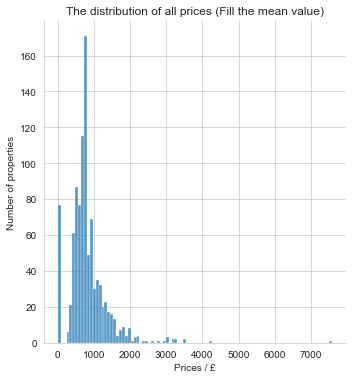
\includegraphics[width=5cm]{price_all_mean}
	\caption{The distribution of prices with mean value filled}
	\label{price_filled}
\end{figure}

\begin{figure*}[h]
	\centering
	\subfigure[Sale Prices]{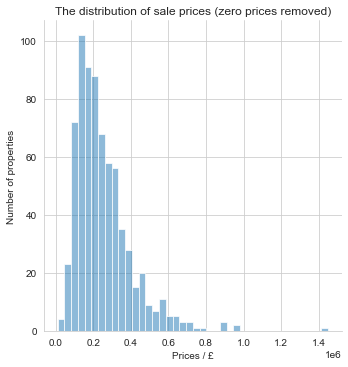
\includegraphics[width=5cm]{price_sale_remove}\label{price_sale_remove}}
	\subfigure[Rental Prices]{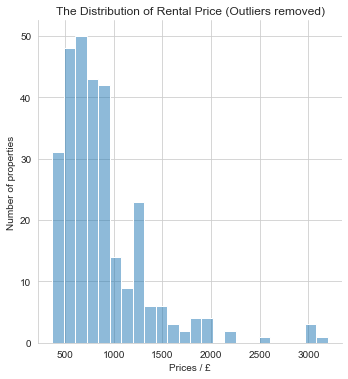
\includegraphics[width=5cm]{price_rental_remove}\label{price_rental_remove}}
	\caption{The distribution of prices with zero prices removed}
	\label{price_removed}
\end{figure*}

\subsection{Create Input Dataset}
The first step in evaluating the behavior of this class is to determine if the categorical features are encoded, and the second test is to inspect whether the missing values are eliminated.
\\

For general information, the first ten rows after preprocessing and their corresponding rows in the original dataset are displayed in figure \ref{general_info}. The categorical features, such as postcode and council tax band, are encoded as numerical values allowing the first test to be passed. In addition, it is evident that the indices in the new dataset are not continuous, indicating that the rows with missing values have been removed. Hence it can pass the second test. 

\begin{figure*}[h]
	\centering
	\subfigure[Original dataset]{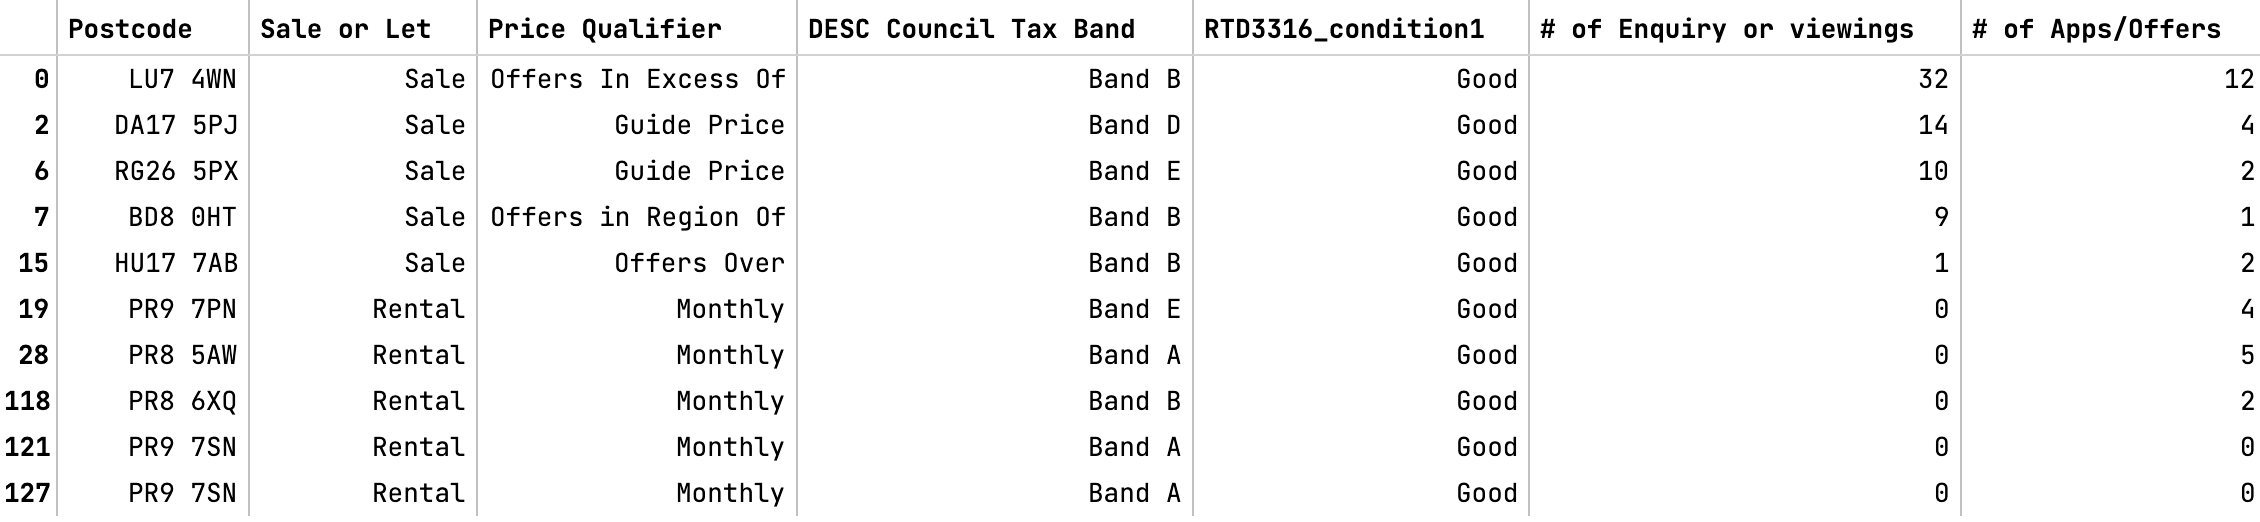
\includegraphics[width=\linewidth]{general_raw}\label{general_raw}}
	\subfigure[Preprocessed dataset]{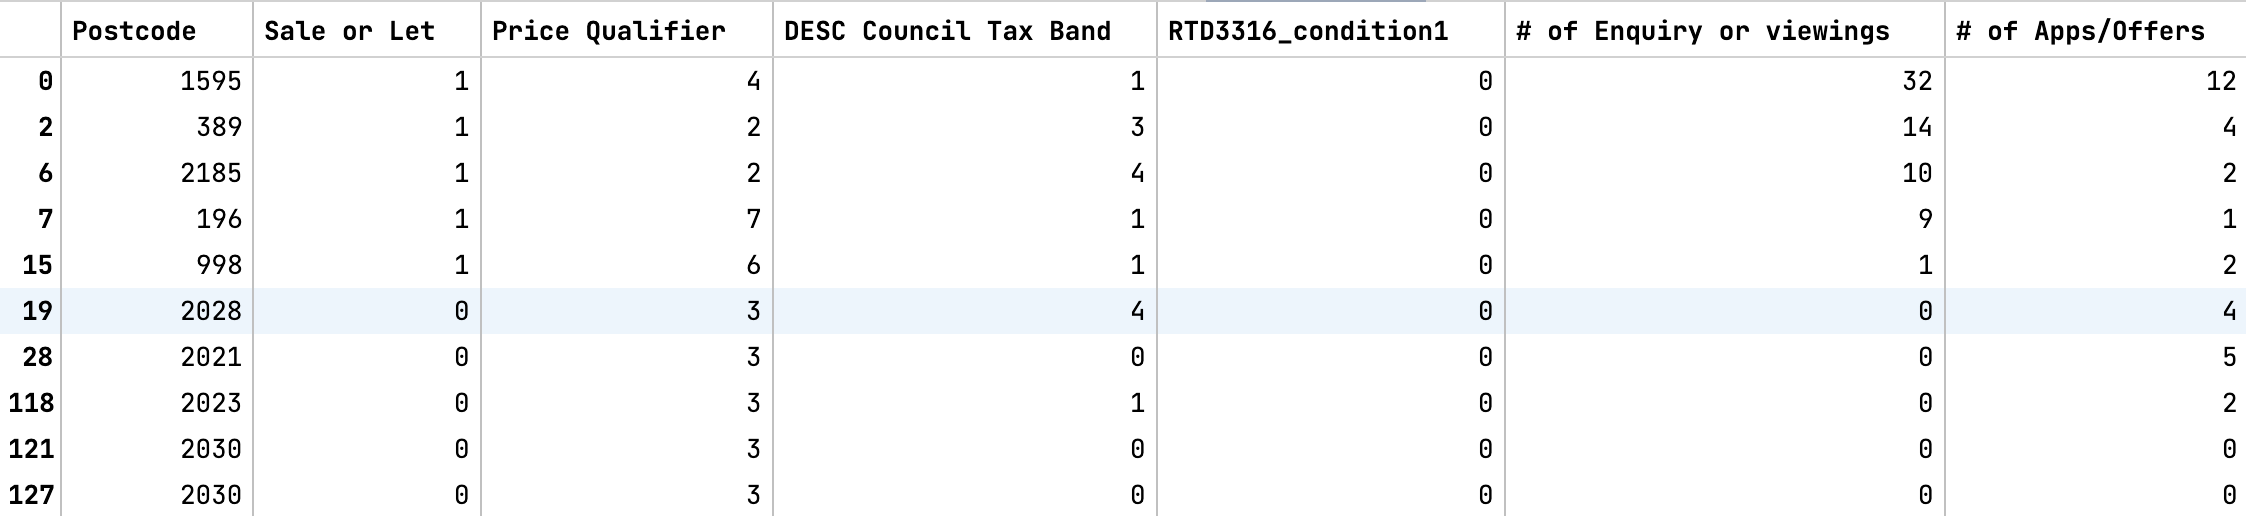
\includegraphics[width=\linewidth]{general_input}\label{general_input}}
	\caption{Comparsion between original and preprocessed dataset}
	\label{general_info}
\end{figure*}

\section{Model Construction}
\subsection{Linear Regression: Predict Price}
The training \& validation losses of this model are depicted in figure \ref{linear_regression_fold_5}, and the model trained in fold two has been chosen for evaluation since it has the best performance. 
\begin{figure*}[h]
	\centering
	\subfigure[Fold 0]{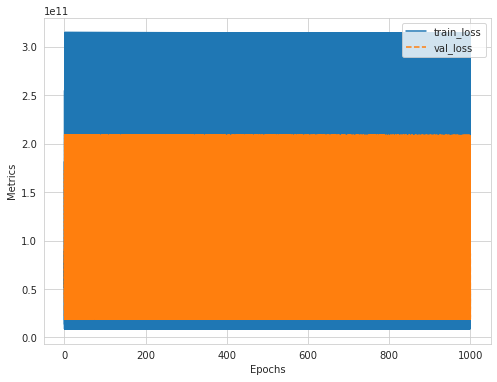
\includegraphics[width=5cm]{linear_regression_fold_0}\label{linear_regression_fold_0}}
	\hfill
	\subfigure[Fold 1]{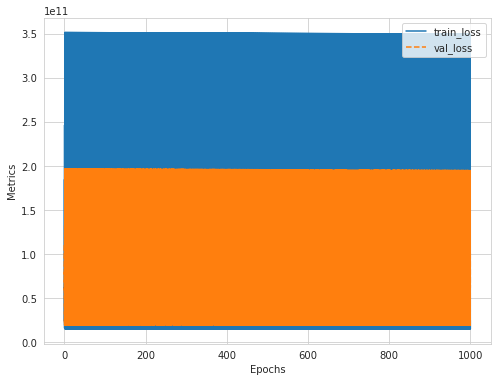
\includegraphics[width=5cm]{linear_regression_fold_1}\label{linear_regression_fold_1}}
	\hfill
	\subfigure[Fold 2]{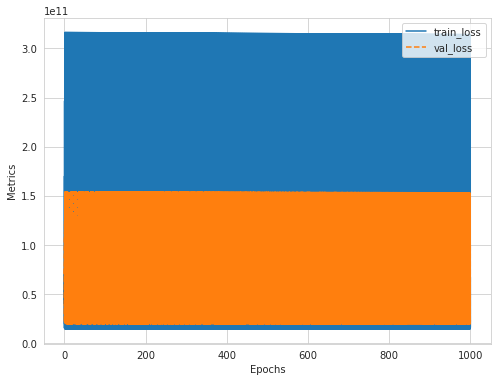
\includegraphics[width=5cm]{linear_regression_fold_2}\label{linear_regression_fold_2}}
	\hfil
	\subfigure[Fold 3]{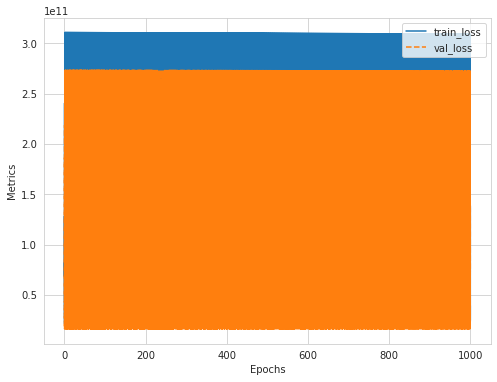
\includegraphics[width=5cm]{linear_regression_fold_3}\label{linear_regression_fold_3}}
	\hfil
	\subfigure[Fold 4]{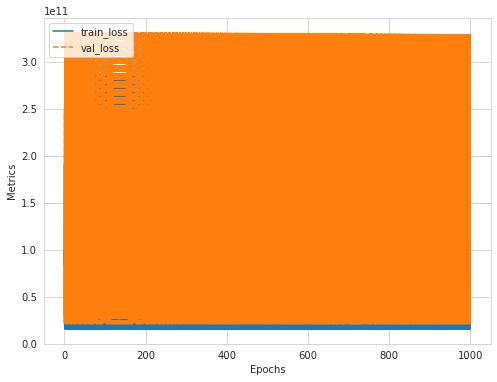
\includegraphics[width=5cm]{linear_regression_fold_4}\label{linear_regression_fold_4}}
	\caption{The training \& validation loss for different folds (linear regression model)}
	\label{linear_regression_fold_5}
\end{figure*}

\begin{table}[h]
	\centering
	\caption{Comparison between truth and model predictions}
	\label{linear_regression_predictions}
	\begin{tabular}{| c | c | c |}
		\hline
		Predicted Price & price & price error  / \%\\ 
		\hline
		940 & 695 & 35.37 \\
		\hline
		4150 & 350000 & 98.81 \\
		\hline
		1790 & 130000 & 98.62 \\
		\hline
		-2101 & 475 & 542.46 \\
		\hline
		1829 & 105000 & 98.25 \\
		\hline
		3058 & 450000 & 99.32 \\
		\hline
		-4289 & 460 & 1032.47 \\
		\hline
		855 & 325000 & 99.74 \\
		\hline
		3255 & 585000 & 99.44 \\
		\hline
		1071 & 900 & 19.10 \\
		\hline
	\end{tabular}
\end{table}

The first ten predictions and the actual prices are displayed in table \ref{linear_regression_predictions}, and it is evident that there are significant differences between the predictions and the truth. Moreover, the model's metrics are as follows, $MAE = 179836$, $MSE = 66601086343$ and $R^2 = -0.9136$. These results demonstrate that a linear regression model cannot extract patterns from the dataset and that neural networks with multiple layers are compulsory.

\subsection{Basic Model: Output Sale Status and Price}
The training and validation losses against epochs for each fold is displayed in figure \ref{sale_fold_5}. For fold zero, the model was overfitting as the training loss was approximately the same after 60 epochs, whereas the validation loss was increasing. If the training stops elrly, then the performance of this model might be the best. For fold one, the model is underfitting as the validation loss keeps decreasing and its performance might be better if it was trained for more epochs. For the next two folds, the performance of the models are the best and should be selected for testing. The model trained from last fold did not learn anything since both training and validation loss is osciliating. 
\\

\begin{figure*}[h]
	\centering
	\subfigure[Fold 0]{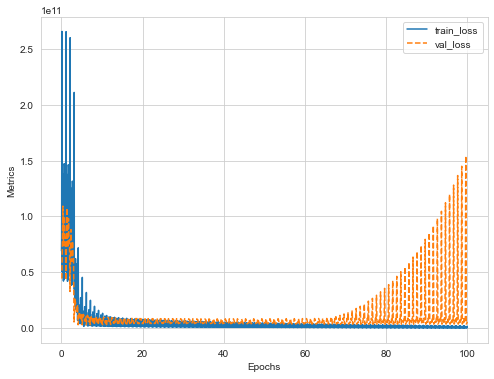
\includegraphics[width=5cm]{sale_fold_5_0}\label{sale_fold_5_0}}
	\hfill
	\subfigure[Fold 1]{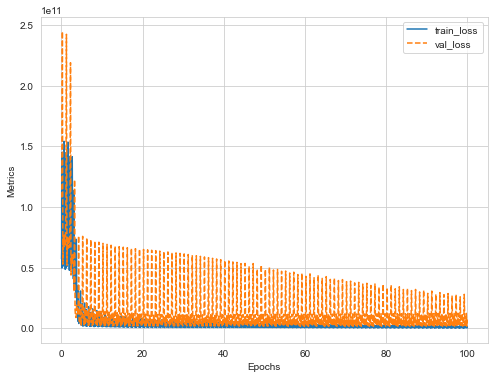
\includegraphics[width=5cm]{sale_fold_5_1}\label{sale_fold_5_1}}
	\hfill
	\subfigure[Fold 2]{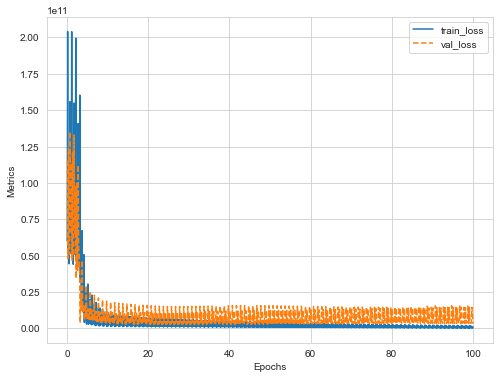
\includegraphics[width=5cm]{sale_fold_5_2}\label{sale_fold_5_2}}
	\hfil
	\subfigure[Fold 3]{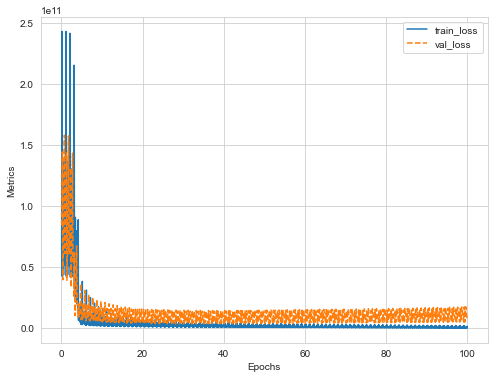
\includegraphics[width=5cm]{sale_fold_5_3}\label{sale_fold_5_3}}
	\hfil
	\subfigure[Fold 4]{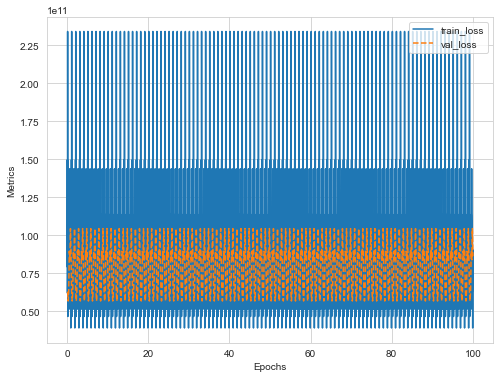
\includegraphics[width=5cm]{sale_fold_5_4}\label{sale_fold_5_4}}
	\caption{The training \& validation loss for different folds}
	\label{sale_fold_5}
\end{figure*}

Based on the performance plot, the model trained in fold 3 was selected. The first ten predictions and true values are shown in table \ref{first_model_predictions}. It is evident that the model only predict one for completeness regardless of the truth values, whereas the predicted prices were better.  
\\

The metrics for price prediction are as follows, $MAE = 57527$, $MSE = 7559964776$ and $R^2 = 0.54$. Comparing this model to the linear regression model demonstrates that the neural network is able to extract patterns from the dataset, resulting in superior performance. 
\\

Figure \ref{confusion_matrix_basic_model} illustrates the confusion matrix of predicting completeness, from which the accuracy, precision, recall, and F1 score are calculated to be 0.638, 0.638, 1, and 0.78, respectively. 
\\

\begin{figure}[h]
	\centering
	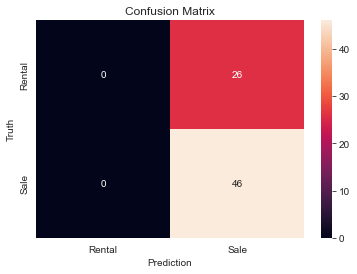
\includegraphics[width=10cm]{confusion_matrix_basic_model}
	\caption{The confusion matrix of the basic model}
	\label{confusion_matrix_basic_model}
\end{figure}

The error result could be caused by loss functions. The completeness is either zero or one, hence the BCE loss was used. For the prices which is greater than zero, the MSE loss was applied. As the model outputs both completeness and prices, the BCE and MSE loss were added to produce a total loss which was then used for backpropagation. However, the BCE loss is small compared with MSE loss. Therefore, the total loss resulted in the model learning more in predicting prices and completeness was ignored. Additionally, another reason causing the wrong predictions on completness was that the price is not input into the model and it is one of the most important factors in real-life transactions. 
\begin{table}[h]
	\centering
	\caption{Comparison between truth and model predictions}
	\label{first_model_predictions}
	\begin{tabular}{| c | c | c | c | c |}
		\hline
		Completed & Price & Predicted completed & Predicted price & Price error  / \%\\ 
		\hline
		1 & 675000 & 1 & 600810 & 10.99 \\
		\hline
		0 & 80000 & 1 & 36130 & 70.16 \\
		\hline
		0 & 90000 & 1 & 53198 & 40.89  \\
		\hline
		0 & 295000 & 1 & 253552 & 14.05  \\
		\hline
		0 & 105000 & 1 & 105753 & 0.72  \\ 
		\hline
		1 & 270000 & 1 & 297239 & 10.09  \\
		\hline
		0 & 115000 & 1 & 124108 & 7.92  \\
		\hline
		1 & 600000 & 1 & 528918 & 11.85  \\
		\hline
		1 & 4000000 & 1 & 376152 & 5.96  \\
		\hline
		0 & 125000 & 1 & 157276 & 25.82  \\
		\hline
	\end{tabular}
\end{table}

\subsection{Basic Model: Predicting Prices}
The training \& validation losses of this model is displayed in figure \ref{all_full_epoch_1000}, and the model from fold one was selected for the evaluation because of its performance. 
\\

The first ten predictions are shown in table \ref{first_model_predictions}, and the metrics of this model are as follows, $MAE = 36538$, $MSE = 4918700785$, and $R^2 = 0.85$. 

\begin{figure*}[h]
	\centering
	\subfigure[Fold 0]{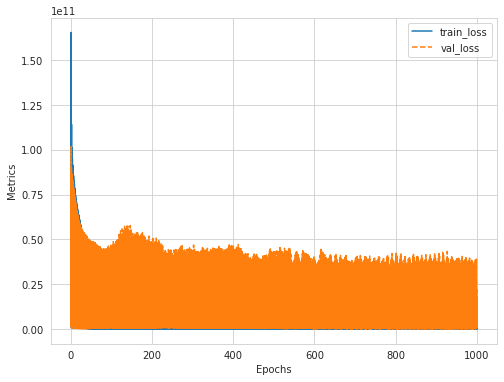
\includegraphics[width=5cm]{all_full_epoch_1000_fold_0}}
	\hfill
	\subfigure[Fold 1]{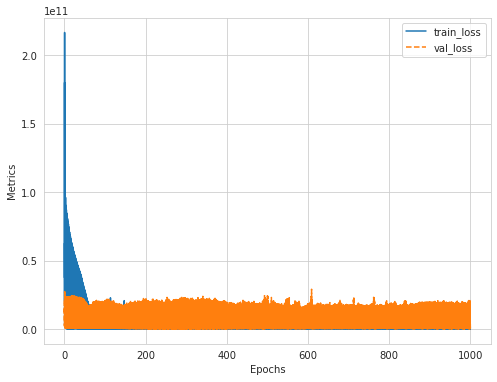
\includegraphics[width=5cm]{all_full_epoch_1000_fold_1}}
	\hfill
	\subfigure[Fold 2]{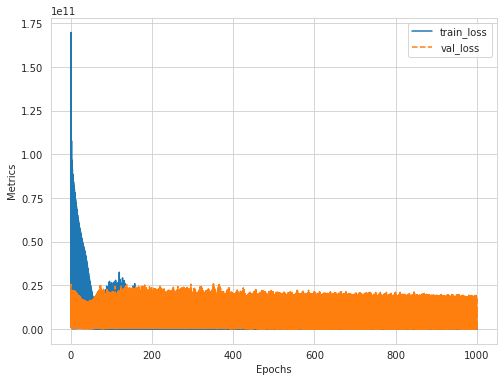
\includegraphics[width=5cm]{all_full_epoch_1000_fold_2}}
	\hfil
	\subfigure[Fold 3]{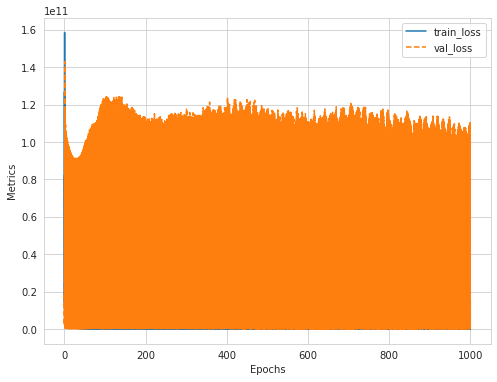
\includegraphics[width=5cm]{all_full_epoch_1000_fold_3}}
	\hfil
	\subfigure[Fold 4]{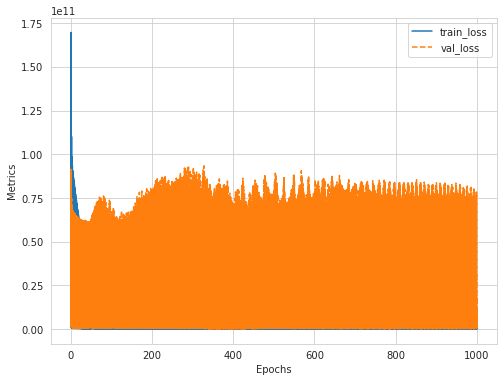
\includegraphics[width=5cm]{all_full_epoch_1000_fold_4}}
	\caption{Training \& validation loss (Model for predicting prices)}
	\label{all_full_epoch_1000}
\end{figure*}

\begin{table}[h]
	\centering
	\caption{Comparison between the true prices and predicted proces}
	\label{basic_model_prediction_price}
	\begin{tabular}{| c | c | c |}
		\hline
		True Price & Predicted Price & Price Error \% \\
		\hline
		0 & 695 & 100 \\
		\hline
		593571 & 350000 & 69.59 \\
		\hline
		177140 & 130000 & 36.26 \\
		\hline
		0 & 475 & 100 \\
		\hline
		156217 & 105000 & 48.77 \\
		\hline
		509198 & 450000 & 13.15 \\
		\hline
		0 & 460 & 100 \\ 
		\hline
		389259 & 325000 & 19.77 \\
		\hline
		571157 & 585000 & 2.36 \\
		\hline
		0 & 900 & 100 \\
		\hline
	\end{tabular}
\end{table}


%%%%%%%%%%%%%%%%%%%%%%%%%%%%%%%%%%%%
\chapter{Conclusion}


%% bibliography
\bibliographystyle{apalike}
\bibliography{proposal}

\end{document}
